\documentclass[aspectratio=43]{beamer}
\usetheme{bydevmar}
%\usefonttheme[onlymath]{serif}

\usepackage{slashed}
\usepackage{datetime}
%\usepackage{slidesphysics}
\graphicspath{{plots/}}
\usepackage{hyperref}
\usepackage{cancel}
% \hypersetup{colorlinks=true, 
%     linkcolor=blue,          % color of internal links (change box color with linkbordercolor)
%     citecolor=black,        % color of links to bibliography
%     filecolor=black,      % color of file links
%     urlcolor=blue    }
% \usepackage{deflamb}
% \usepackage{color, colortbl}
% \usepackage{tikz}
%\usepackage{userdef}
\usepackage[absolute,overlay]{textpos}
\def\Put(#1,#2)#3{\leavevmode\makebox(0,0){\put(#1,#2){#3}}}

\def\mydate{\leavevmode\hbox{\the\year-\twodigits\month-\twodigits\day}}
\def\twodigits#1{\ifnum#1<10 0\fi\the#1}

\newcommand\Wider[2][3em]{%
\makebox[\linewidth][c]{%
  \begin{minipage}{\dimexpr\textwidth+#1\relax}
  \raggedright
  \centering#2
  \end{minipage}%
  }%
}

\def\meetingname{Mathématiques pour l'économie II}
\def\presenters{Présentateurs:   
            ABATOUR Driss 
            \\ \hspace{2.7cm} GAJJA Nour Eddin
            \\ \hspace{3.2cm} BOUHLALI Abdelfattah }
\def\supervisor{Encadrent: Z. RAZIKI}

\title[\meetingname]{Bâle et la loi Dodd-Frank}
%\institute[FPO]{intitute name}
\institute[FPO]{Faculté Polydisciplinaire de Ouarzazate}
\date[\mydate]{\meetingname\\\today}




% Define a custom command for section frame
\newcommand{\sectionframe}[1]{%
  \begin{frame}
    \begin{center}
      \LARGE \insertsectionhead
    \end{center}
  \end{frame}
}

% Add section frame at the beginning of each section
\AtBeginSection[]{
  \sectionframe{\thesection.~\insertsection}
}




\begin{document}
\begin{frame}[plain,t]
\titlepage
\begin{textblock*}{\linewidth}(1cm,6cm) % Adjust the position of the text block as needed
    \centering
    \small \presenters \\
    \small \supervisor
\end{textblock*}
\end{frame}

%The next statement creates the title page.
\begin{frame}
\frametitle{Contents}
\tableofcontents
\end{frame}
%------------------------------------------------------------
% -Introduction
\section{Concepts Introductifs}



\begin{frame}{Détection de fraude}
    \begin{center}
        \colorbox{white}{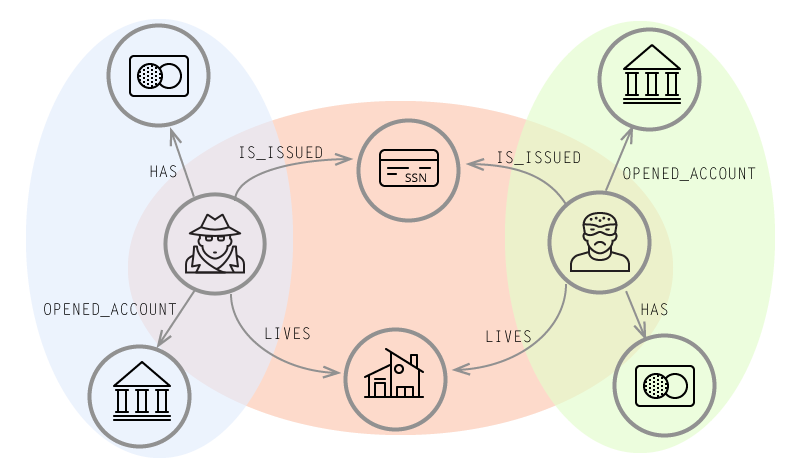
\includegraphics[width=0.8\textwidth]{img/usecase-fraud.png}}
\end{center}
\end{frame}


\begin{frame}
\frametitle{Connectivité dans les Graphes : Variétés, Implications et Exemples}
    \begin{tcolorbox}[colback=orange!10,colframe=orange!100!black,
        title=La connectivité dans les graphes]
        La connectivité dans les graphes a des implications variées dans de nombreux domaines, tels que les réseaux informatiques, la planification urbaine et la biologie. Elle est définie comme suit :
        \begin{itemize}
            \item \textbf{Connectivité de sommets ($\kappa$)}: Le nombre minimum de sommets dont la suppression entraîne un graphe non connexe ou réduit le graphe à un seul sommet.
            \item \textbf{Connectivité d'arêtes ($\lambda$)}: Le nombre minimum d'arêtes dont la suppression rend le graphe non connexe.
        \end{itemize}
        Ces deux mesures sont liées par l'inégalité suivante :
        $$ \kappa(G) \leq \lambda(G) \leq \delta(G) $$
        où $\delta(G)$ est le degré minimum d'un sommet dans le graphe $G$.
    \end{tcolorbox}
\end{frame}

\begin{frame}{	CLI Neo4j Command Line Interface}
  \begin{block}{cli neo4 j}
    	CLI Neo4j (Command Line Interface) :
\begin{itemize}
   
	\item Pour exécuter une requête Cypher, vous pouvez utiliser la commande cypher suivie de votre requête. Par exemple : cypher "MATCH (n) RETURN n"
\item	Pour gérer les utilisateurs et les autorisations, vous pouvez utiliser les commandes user et role.
\item	Pour importer des données, utilisez la commande import.
\item	Pour surveiller et configurer votre instance Neo4j, vous pouvez utiliser des commandes telles que info, metrics, set, etc.
\end{itemize}
  \end{block}
  
\end{frame}
\begin{frame}
\frametitle{Exploration de la Connectivité des Graphes : Théorème de Menger}
\begin{tcolorbox}[colback=orange!10,colframe=orange!100!black,
    title=\textbf{Théorème de Menger}]
    Le théorème de Menger est un résultat fondamental en théorie des graphes qui établit une relation entre la connectivité locale et globale d'un graphe. Il stipule que pour deux sommets non adjacents \( u \) et \( v \) dans un graphe, le nombre minimum de sommets à supprimer pour séparer \( u \) et \( v \) est égal au nombre maximum de chemins indépendants de \( u \) à \( v \).
    
    Formellement, la formule mathématique est donnée par :
    $$ \kappa(u,v) = \max \{ \text{nombre de chemins indépendants de } u \text{ à } v \} $$
    où \( \kappa(u,v) \) représente la connectivité entre les sommets \( u \) et \( v \).
\end{tcolorbox}
\end{frame}

\begin{frame}
\frametitle{Application Pratique : Théorème de Menger}
\begin{tcolorbox}[colback=orange!10,colframe=orange!100!black,
    title=\textbf{Exemple du Théorème de Menger}]
    Considérons un graphe où les sommets \( A \) et \( B \) ne sont pas adjacents. Selon le théorème de Menger, pour déterminer le nombre minimum de sommets à supprimer pour séparer \( A \) de \( B \), nous devons trouver le nombre maximum de chemins indépendants de \( A \) à \( B \).

    Supposons qu'il y ait trois chemins indépendants entre \( A \) et \( B \). Alors, selon le théorème de Menger, nous devons supprimer au moins trois sommets pour séparer \( A \) de \( B \).

    La formule mathématique s'applique comme suit :
    $$ \kappa(A,B) = 3 $$
    Ce qui signifie que la connectivité \( \kappa \) entre \( A \) et \( B \) est de trois, et donc trois est le nombre minimum de sommets à supprimer pour les séparer.
\end{tcolorbox}
\end{frame}




\begin{frame}{ \textbf{Example  Importation à partir de fichiers CSV}}
\textit{}{\textbf{Fichier CSV :}}  
    \begin{center}
        \begin{tabular}{|l|l|l|}
            \hline
           name & ville& age \\
            \hline
            hassan & casa& 25 \\
           walid & fes  & 23 \\
           fatima & agadir & 65 \\
            \hline
        \end{tabular}
    \end{center}
    
 \begin{block}{cypher}
 LOAD CSV WITH HEADERS FROM 'file:///employees.csv' AS row
CREATE (:person { name: row.name, ville: row.ville, age: toInteger(row.age)})

  \end{block}
\end{frame}    
\begin{frame}{La loi Dodd-Frank et son impact sur la réglementation Q}
   La loi Dodd-Frank a abrogé le règlement Q, autorisant les banques à payer des intérêts sur les dépôts à vue pour la première fois depuis plus de 70 ans. Ce changement a été perçu comme une évolution positive par beaucoup, car il offre aux consommateurs davantage d’options pour épargner et gagner des intérêts. Cependant, certains craignaient que l'abrogation du règlement Q puisse également conduire à une prise de risque accrue de la part des banques, dans la mesure où elles seraient désormais en mesure d'offrir des taux de dépôt plus élevés pour attirer les clients. 
\end{frame}
\begin{frame}
\frametitle{Définitions Fondamentales des Graphes}

\begin{tcolorbox}[colback=orange!10,colframe=orange!100!black,
    title=Un Cycle]
    Un \textbf{Cycle} est un chemin qui commence et se termine au même sommet.
\end{tcolorbox}

\begin{figure}[H]
    \centering
    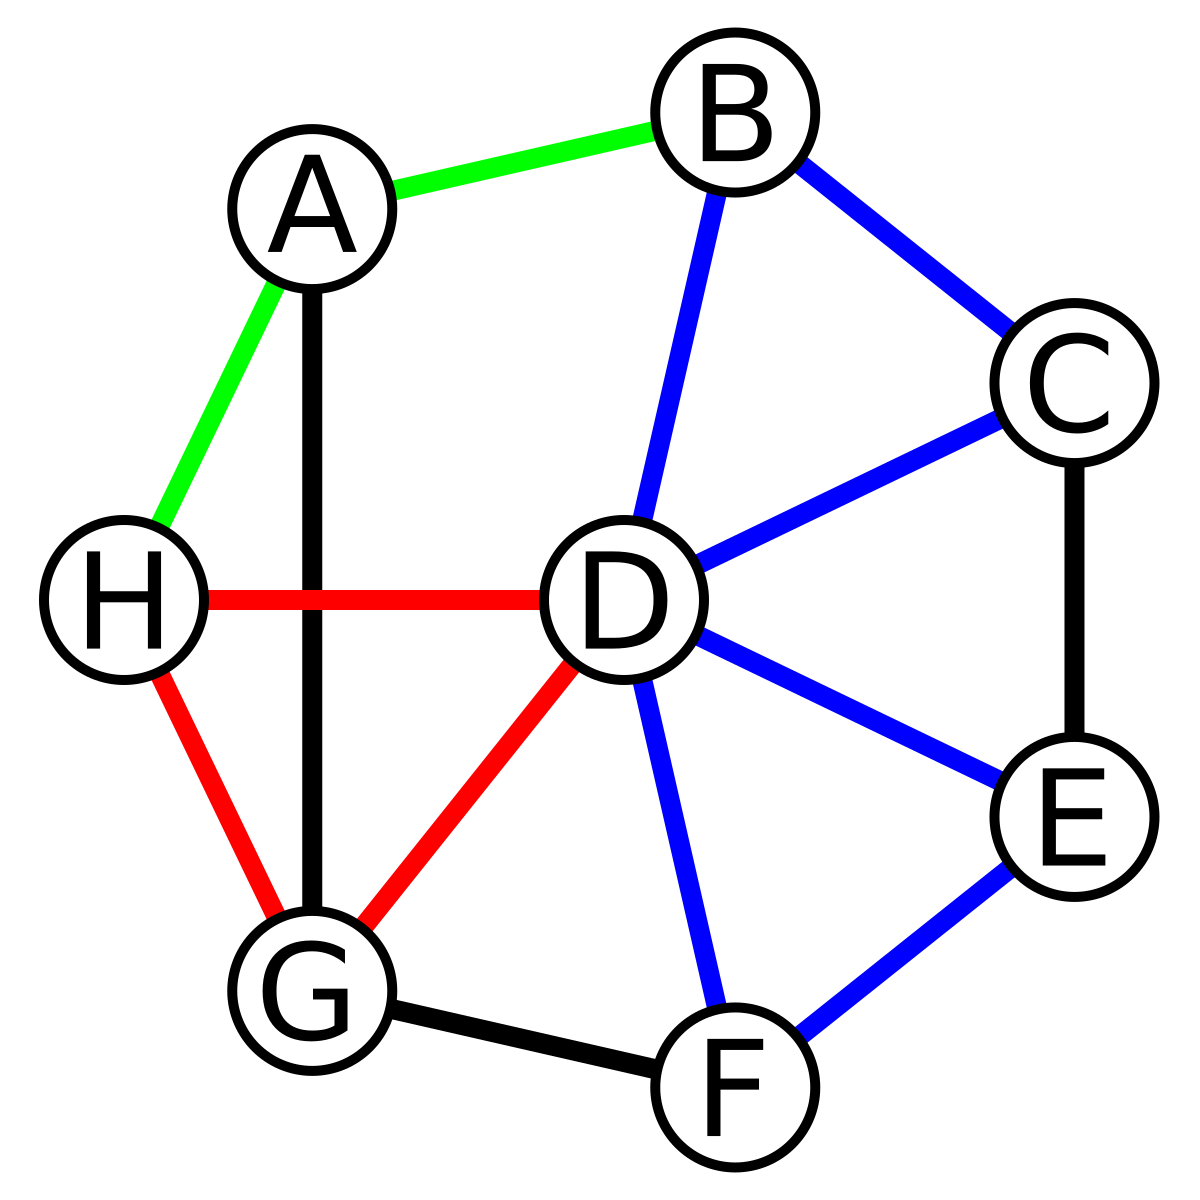
\includegraphics[width=0.5 \textwidth]{Figures/cycle.png}
    \caption{Un Cycle}
    \label{fig:Un Cycle}
\end{figure}

\end{frame}

\begin{frame}{les instruments financiers et la loi Dodd-Frank }


Avant Dodd-Frank, les instruments financiers manquaient de régulation, exposant à l'opacité et aux abus. Les dérivés étaient utilisés sans contrôle, alimentant l'instabilité. Dodd-Frank a transformé cela en imposant la transparence des dérivés, renforçant la surveillance avec des organismes comme le FSOC et protégeant les consommateurs. Les exigences plus strictes ont également renforcé la stabilité financière. Ainsi, Dodd-Frank a rendu les instruments financiers plus sûrs et mieux réglementés.
\end{frame}
\begin{frame}{Exécution de requêtes en direct}
  \begin{block}{Trouver tous les joueurs d'une équipe}
    \begin{itemize}
      \item MATCH (j:Joueur)-[:JOUE\_POUR]->(e:Equipe {nom: 'PSG'});
      \item RETURN j.nom, j.prenom, j.age;
    \end{itemize}
    Cette requête retourne les noms, prénoms et âges de tous les joueurs qui jouent pour le PSG.
  \end{block}
  \begin{block}{Trouver l'entraîneur d'une équipe}
    \begin{itemize}
      \item MATCH (e:Equipe {nom: 'FCB'})<-[:ENTRAINE]-(entraineur);
      \item RETURN entraineur.nom;
    \end{itemize}
    Cette requête retourne le nom de l'entraîneur du FC Barcelone.
  \end{block}
\end{frame}

% - Les Accords Basel
\section{Les Accords de Bâle}


\begin{frame}{historique des événements liés à la réglementation du système bancaire}
\begin{table}[htbp]
    \centering
    \begin{tabular}{|c|p{4cm}|p{4cm}|}
        \hline
        \textbf{Année} & \textbf{Événement} & \textbf{Conséquences} \\
        \hline
        1974 & Faillite de la Herstatt Bank & Crise financière en Europe \\
             & Création du Comité de Bâle & Établissement de normes de régulation \\
        \hline
        1975 & Concordat de Bâle & Exigences minimales de fonds propres \\
        \hline
        1995-1998 & Crise mexicaine, crise asiatique & Élaboration de Bâle II \\
        \hline
        2007-2008 & Crise des subprimes, faillite de Lehman Brothers & Élaboration de Bâle III \\
        \hline
        2017 & Finalisation de Bâle III & Mise en œuvre des accords de Bâle III \\
        \hline
    \end{tabular}
   % \caption{Chronologie des crises du système bancaire}
    %\label{tab:crises_bancaires}
\end{table}
\end{frame}

\begin{frame}{La création du Comité de Bâle}
    \begin{figure}[h]
        \centering
        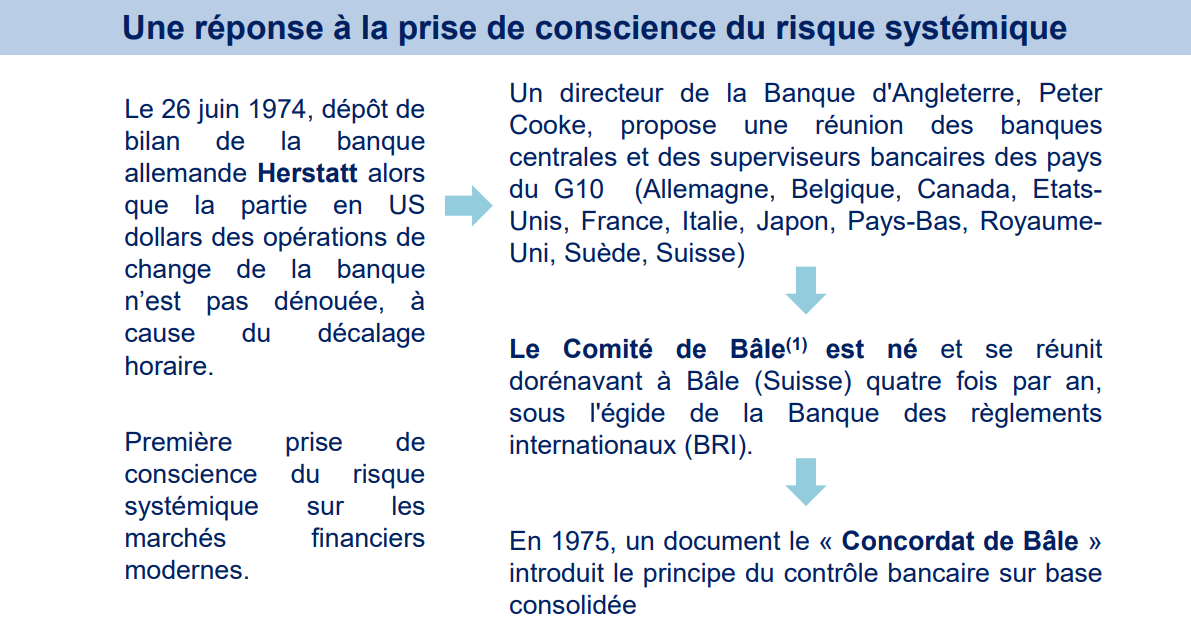
\includegraphics[scale=0.45]{Frames/Les Accords de Bale/p2.png}
        %\caption{Une réponse à la prise de conscience du risque systémique}
        %\label{fig:accords_bale_2}
    \end{figure}
\end{frame}


\begin{frame}{Le 1er accord de Bâle, dit ratio Cooke}
    \begin{figure}[h]
        \centering
        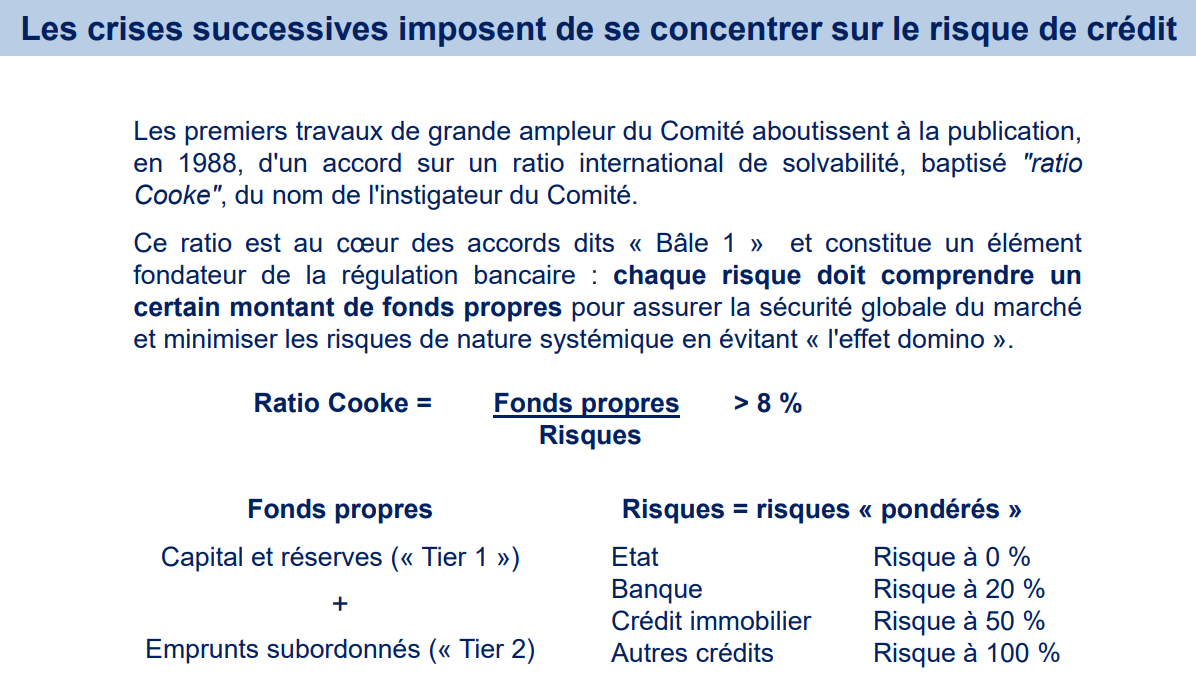
\includegraphics[scale=0.45]{Frames/Les Accords de Bale/p3.png}
       % \caption{Les crises successives imposent de se concentrer sur le risque de crédit}
        %\label{fig:accords_bale_2}
    \end{figure}
\end{frame}


\begin{frame}{Bâle 2 : les 3 piliers de la régulation bancaire}
    \begin{figure}[h]
        \centering
        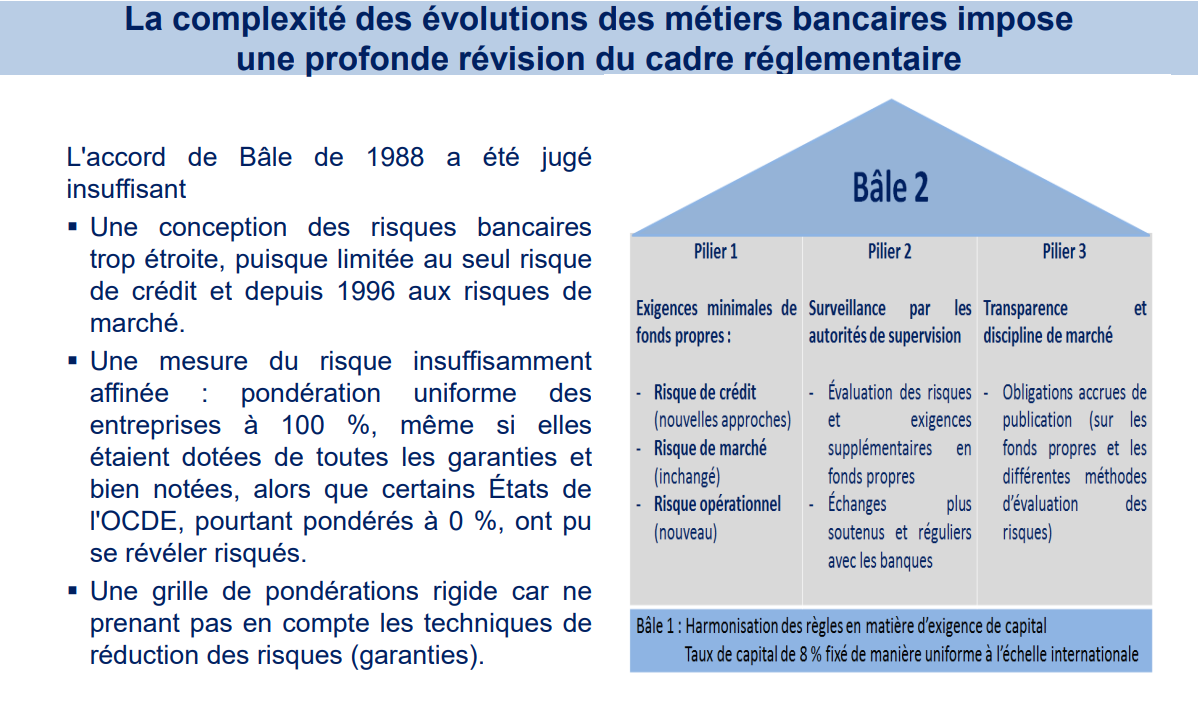
\includegraphics[scale=0.47]{Frames/Les Accords de Bale/p4.png}
        %\caption{La complexité des évolutions des métiers bancaires}
        %\label{fig:accords_bale_2}
    \end{figure}
\end{frame}


\begin{frame}{Bâle 3 : répondre à la crise de 2007/2008 et 2010}
    \begin{figure}[h]
        \centering
        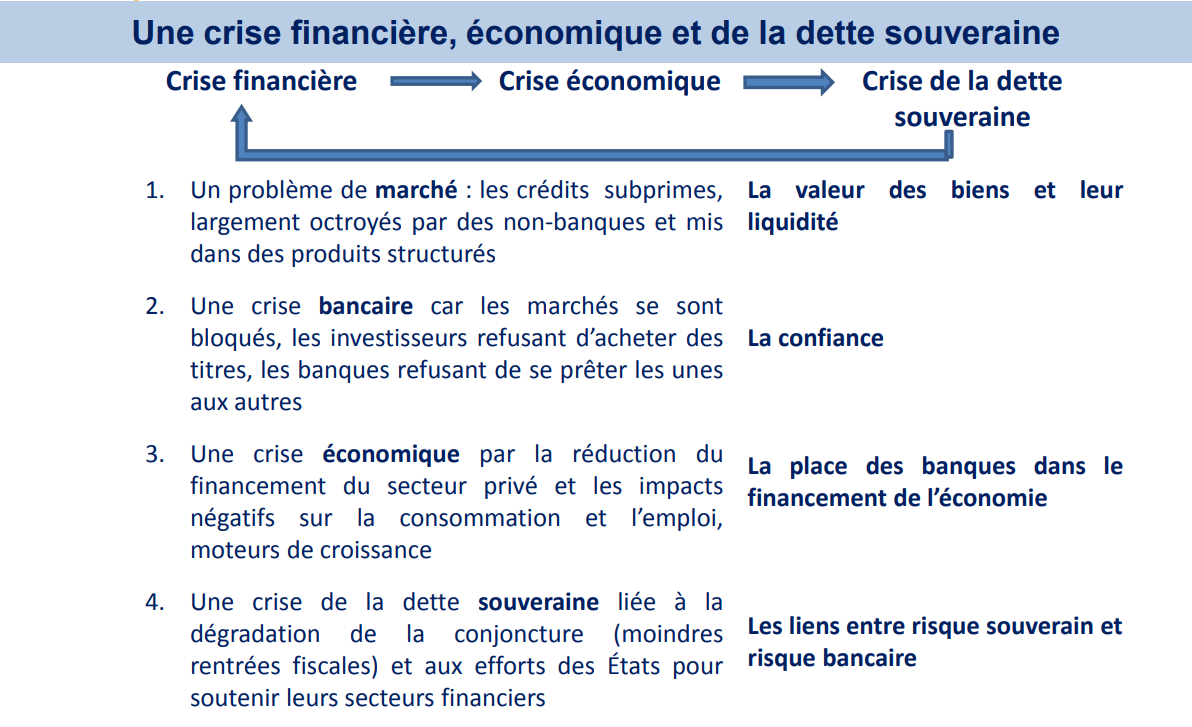
\includegraphics[scale=0.4]{Frames/Les Accords de Bale/b3.png}
        %\caption{Une crise financière, économique et de la dette souveraine}
        %\label{fig:accords_bale_2}
    \end{figure}
\end{frame}







\begin{frame}{Bâle 3 : répondre à la crise de 2007/2008 et 2010}
    \begin{figure}[h]
        \centering
        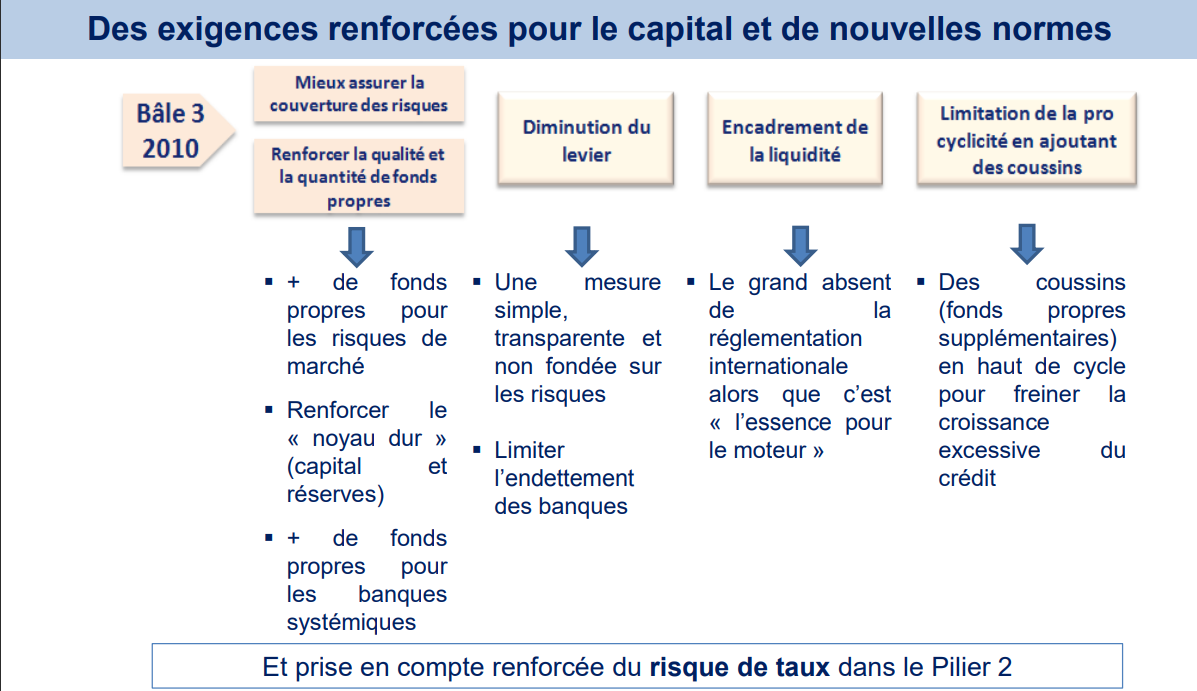
\includegraphics[scale=0.43]{Frames/Les Accords de Bale/b6.png}
        %\caption{Quatre normes quantitatives au lieu d’une seul }
        %\label{fig:accords_bale_2}
    \end{figure}
\end{frame}




\begin{frame}{Finalisation de Bâle 3}
    \begin{figure}[h]
        \centering
        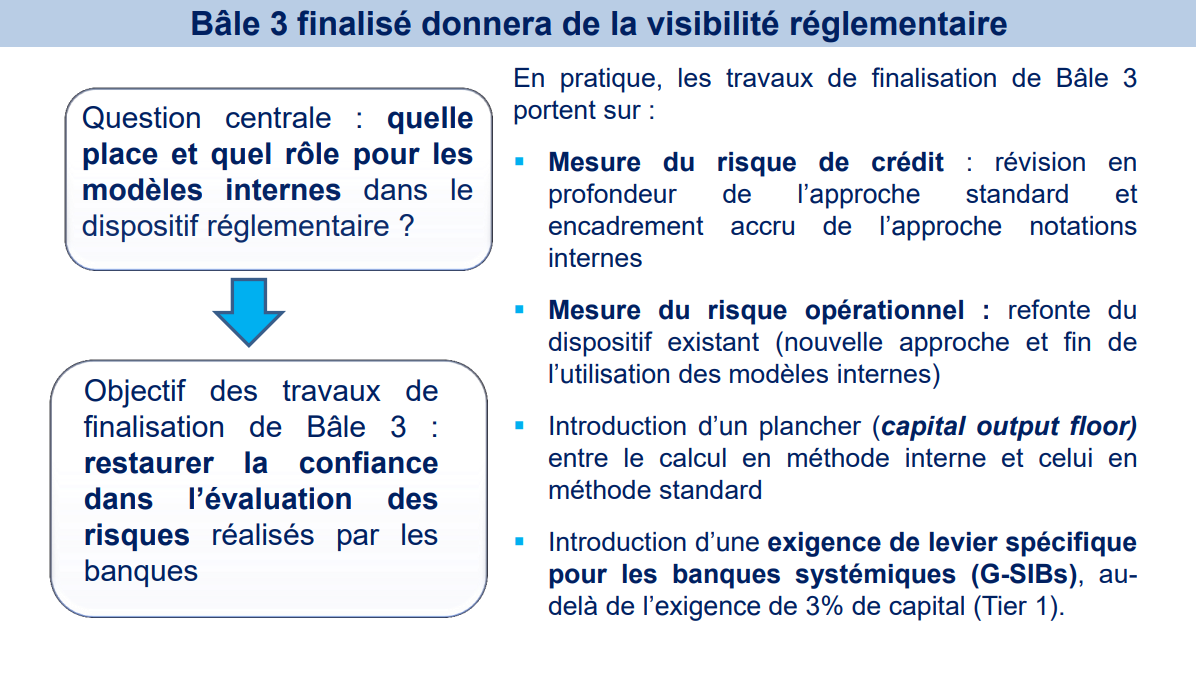
\includegraphics[scale=0.43]{Frames/Les Accords de Bale/b7.png}
       % \caption{Combler les insuffisances et les défauts  de la réglementation Bâle2 }
        %\label{fig:accords_bale_2}
    \end{figure}
\end{frame}


% - La Loi Dodd Frank
\section{La Loi Dodd-Frank}
\begin{frame}{Règlement Q et loi Dodd Frank }
    
\textbf{introduction à la loi Dodd-Frank et aurèglement Q}
\\


La loi Dodd-frank a été adoptée par le Congrès américain en 2010, à la suite de la crise financière de 2008. La loi visait à prévenir une nouvelle crise financière en réglementant le secteur financier et en protégeant les consommateurs. L'une des dispositions clés de la loi Dodd-Frank est le règlement Q, qui régit le paiement des intérêts sur les dépôts par les banques.
   
\end{frame}
\begin{frame}{Détection de fraude}
    \begin{center}
        \colorbox{white}{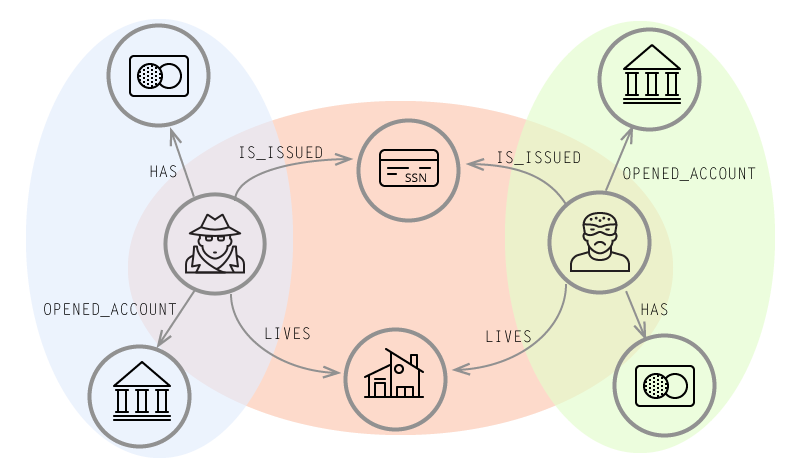
\includegraphics[width=0.8\textwidth]{img/usecase-fraud.png}}
\end{center}
\end{frame}


\begin{frame}
\frametitle{Définitions Fondamentales des Graphes}

\begin{tcolorbox}[colback=orange!10,colframe=orange!100!black,
    title=Un Cycle]
    Un \textbf{Cycle} est un chemin qui commence et se termine au même sommet.
\end{tcolorbox}

\begin{figure}[H]
    \centering
    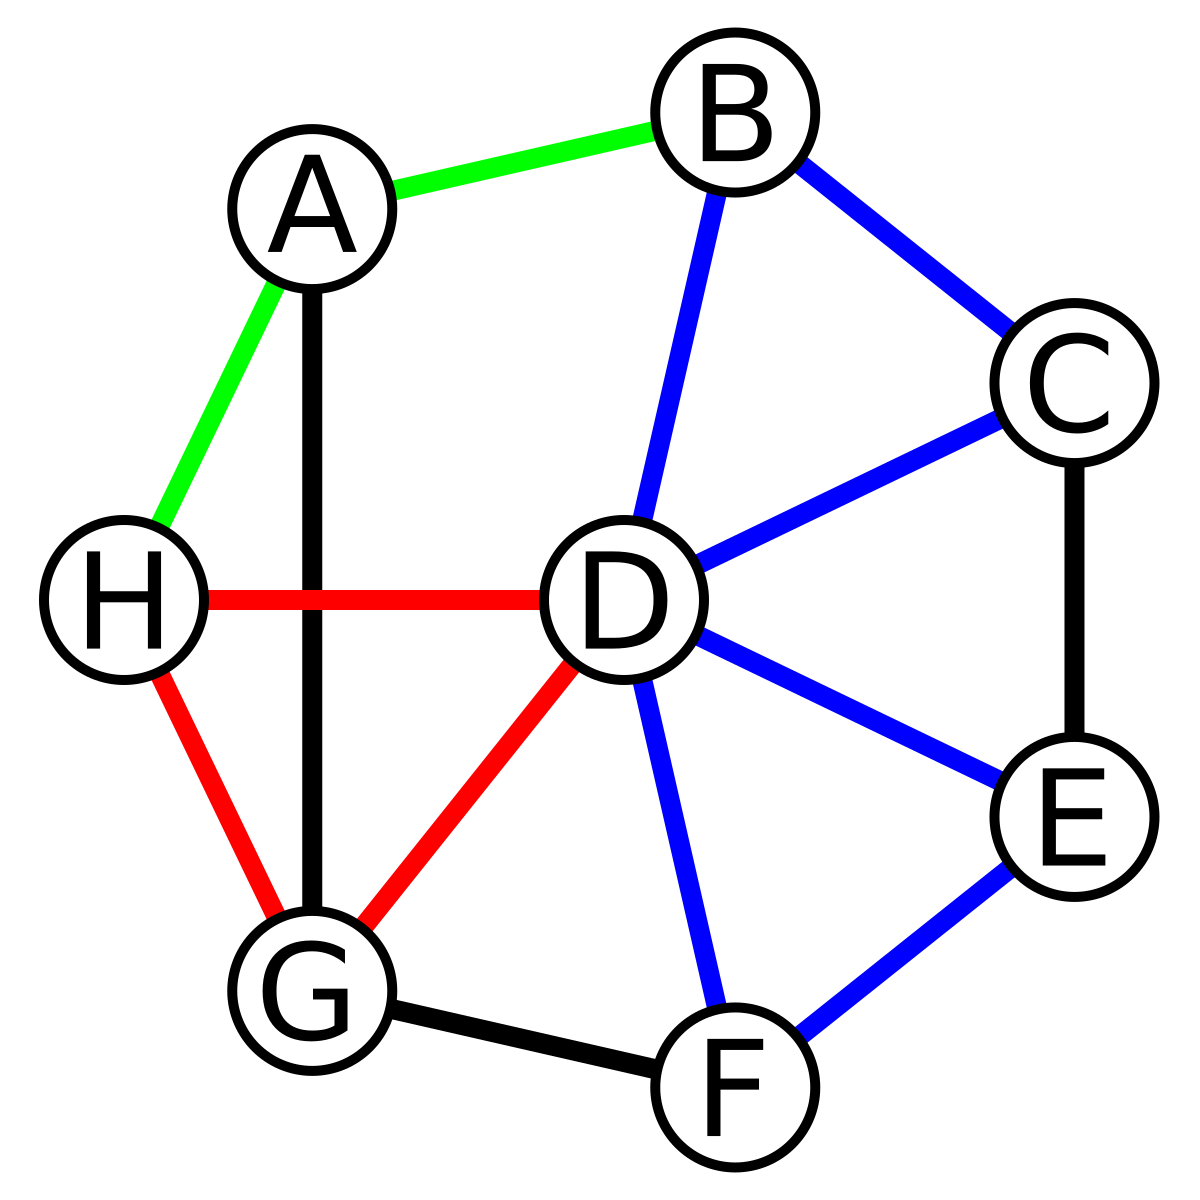
\includegraphics[width=0.5 \textwidth]{Figures/cycle.png}
    \caption{Un Cycle}
    \label{fig:Un Cycle}
\end{figure}

\end{frame}

\begin{frame}{La loi Dodd-Frank et son impact sur la réglementation Q}
   La loi Dodd-Frank a abrogé le règlement Q, autorisant les banques à payer des intérêts sur les dépôts à vue pour la première fois depuis plus de 70 ans. Ce changement a été perçu comme une évolution positive par beaucoup, car il offre aux consommateurs davantage d’options pour épargner et gagner des intérêts. Cependant, certains craignaient que l'abrogation du règlement Q puisse également conduire à une prise de risque accrue de la part des banques, dans la mesure où elles seraient désormais en mesure d'offrir des taux de dépôt plus élevés pour attirer les clients. 
\end{frame}
\begin{frame}{les instruments financiers et la loi Dodd-Frank }


Avant Dodd-Frank, les instruments financiers manquaient de régulation, exposant à l'opacité et aux abus. Les dérivés étaient utilisés sans contrôle, alimentant l'instabilité. Dodd-Frank a transformé cela en imposant la transparence des dérivés, renforçant la surveillance avec des organismes comme le FSOC et protégeant les consommateurs. Les exigences plus strictes ont également renforcé la stabilité financière. Ainsi, Dodd-Frank a rendu les instruments financiers plus sûrs et mieux réglementés.
\end{frame}
\begin{frame}
\frametitle{Connectivité dans les Graphes : Variétés, Implications et Exemples}
    \begin{tcolorbox}[colback=orange!10,colframe=orange!100!black,
        title=La connectivité dans les graphes]
        La connectivité dans les graphes a des implications variées dans de nombreux domaines, tels que les réseaux informatiques, la planification urbaine et la biologie. Elle est définie comme suit :
        \begin{itemize}
            \item \textbf{Connectivité de sommets ($\kappa$)}: Le nombre minimum de sommets dont la suppression entraîne un graphe non connexe ou réduit le graphe à un seul sommet.
            \item \textbf{Connectivité d'arêtes ($\lambda$)}: Le nombre minimum d'arêtes dont la suppression rend le graphe non connexe.
        \end{itemize}
        Ces deux mesures sont liées par l'inégalité suivante :
        $$ \kappa(G) \leq \lambda(G) \leq \delta(G) $$
        où $\delta(G)$ est le degré minimum d'un sommet dans le graphe $G$.
    \end{tcolorbox}
\end{frame}

\begin{frame}{	CLI Neo4j Command Line Interface}
  \begin{block}{cli neo4 j}
    	CLI Neo4j (Command Line Interface) :
\begin{itemize}
   
	\item Pour exécuter une requête Cypher, vous pouvez utiliser la commande cypher suivie de votre requête. Par exemple : cypher "MATCH (n) RETURN n"
\item	Pour gérer les utilisateurs et les autorisations, vous pouvez utiliser les commandes user et role.
\item	Pour importer des données, utilisez la commande import.
\item	Pour surveiller et configurer votre instance Neo4j, vous pouvez utiliser des commandes telles que info, metrics, set, etc.
\end{itemize}
  \end{block}
  
\end{frame}
\begin{frame}
\frametitle{Exploration de la Connectivité des Graphes : Théorème de Menger}
\begin{tcolorbox}[colback=orange!10,colframe=orange!100!black,
    title=\textbf{Théorème de Menger}]
    Le théorème de Menger est un résultat fondamental en théorie des graphes qui établit une relation entre la connectivité locale et globale d'un graphe. Il stipule que pour deux sommets non adjacents \( u \) et \( v \) dans un graphe, le nombre minimum de sommets à supprimer pour séparer \( u \) et \( v \) est égal au nombre maximum de chemins indépendants de \( u \) à \( v \).
    
    Formellement, la formule mathématique est donnée par :
    $$ \kappa(u,v) = \max \{ \text{nombre de chemins indépendants de } u \text{ à } v \} $$
    où \( \kappa(u,v) \) représente la connectivité entre les sommets \( u \) et \( v \).
\end{tcolorbox}
\end{frame}

\begin{frame}
\frametitle{Application Pratique : Théorème de Menger}
\begin{tcolorbox}[colback=orange!10,colframe=orange!100!black,
    title=\textbf{Exemple du Théorème de Menger}]
    Considérons un graphe où les sommets \( A \) et \( B \) ne sont pas adjacents. Selon le théorème de Menger, pour déterminer le nombre minimum de sommets à supprimer pour séparer \( A \) de \( B \), nous devons trouver le nombre maximum de chemins indépendants de \( A \) à \( B \).

    Supposons qu'il y ait trois chemins indépendants entre \( A \) et \( B \). Alors, selon le théorème de Menger, nous devons supprimer au moins trois sommets pour séparer \( A \) de \( B \).

    La formule mathématique s'applique comme suit :
    $$ \kappa(A,B) = 3 $$
    Ce qui signifie que la connectivité \( \kappa \) entre \( A \) et \( B \) est de trois, et donc trois est le nombre minimum de sommets à supprimer pour les séparer.
\end{tcolorbox}
\end{frame}




\begin{frame}{ \textbf{Example  Importation à partir de fichiers CSV}}
\textit{}{\textbf{Fichier CSV :}}  
    \begin{center}
        \begin{tabular}{|l|l|l|}
            \hline
           name & ville& age \\
            \hline
            hassan & casa& 25 \\
           walid & fes  & 23 \\
           fatima & agadir & 65 \\
            \hline
        \end{tabular}
    \end{center}
    
 \begin{block}{cypher}
 LOAD CSV WITH HEADERS FROM 'file:///employees.csv' AS row
CREATE (:person { name: row.name, ville: row.ville, age: toInteger(row.age)})

  \end{block}
\end{frame}    











% -Conclusion


\section{Conclusion}
\begin{frame}
\frametitle{Conclusion}
\begin{itemize}
    \item Le \textbf{théorème de Menger} est un concept central en théorie des graphes, essentiel pour comprendre la connectivité.
    \item Ses applications sont vastes, touchant des domaines tels que les réseaux informatiques, l'urbanisme et la biologie.
    \item La capacité à identifier les chemins indépendants et les points de vulnérabilité dans les réseaux peut conduire à des améliorations significatives dans la conception et la résilience des systèmes.
    \item Les concepts de connectivité et de distance dans les graphes continueront d'être des sujets de recherche pertinents pour résoudre des problèmes complexes dans diverses disciplines.
\end{itemize}
\textbf{Perspectives :} La poursuite de l'étude des graphes et de leurs propriétés est cruciale pour le développement de technologies et d'infrastructures plus robustes et efficaces à l'avenir.
\end{frame}







%}
%\setbeamercolor{background canvas}{bg=violet}
\setbeamercolor{background canvas}{bg=BYDEVMaize}
\begin{frame}[plain,t]
\vspace{100pt}
\centering

\includegraphics[width=0.6\textwidth]{Assets/fpo_logo.png}
\end{frame}
\end{document}
